\documentclass[tikz,border=5pt]{standalone}
\usepackage{tikz}
\usepackage{lmodern}
\usetikzlibrary{shapes,arrows,positioning,calc,fit}

\begin{document}
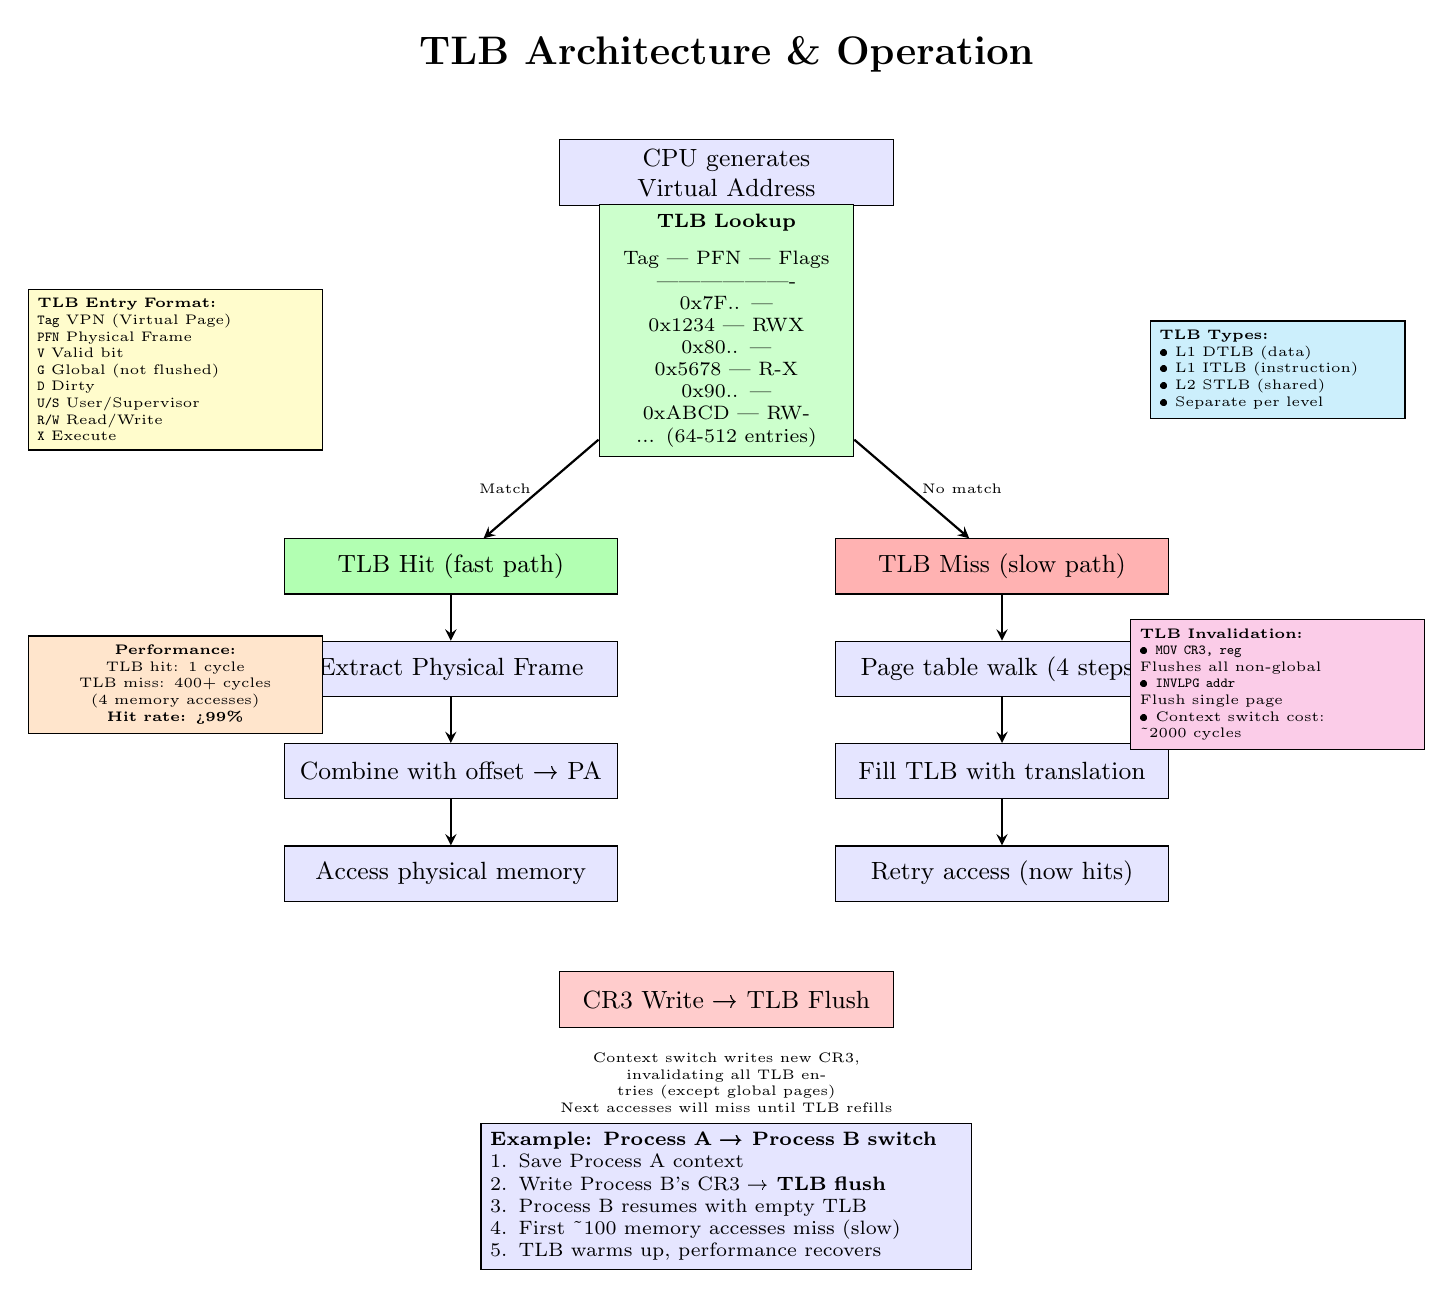
\begin{tikzpicture}[
    node distance=0.9cm,
    box/.style={rectangle, draw, fill=blue!10, text width=4cm, align=center, minimum height=0.7cm, font=\small},
    cache/.style={rectangle, draw, fill=green!20, text width=3cm, align=center, minimum height=0.7cm, font=\scriptsize},
    arrow/.style={->,>=stealth,thick}
]

% Title
\node[font=\Large\bfseries] at (0,0) {TLB Architecture \& Operation};

% CPU generates VA
\node[box] (va) at (0,-1.5) {CPU generates Virtual Address};

% TLB lookup
\node[cache, minimum height=2.5cm] (tlb) at (0,-3.5) {
    \textbf{TLB Lookup}\\
    \vspace{0.2cm}
    Tag | PFN | Flags\\
    -------------------\\
    0x7F.. | 0x1234 | RWX\\
    0x80.. | 0x5678 | R-X\\
    0x90.. | 0xABCD | RW-\\
    ... (64-512 entries)
};

% TLB hit path
\node[box, fill=green!30] (hit) at (-3.5,-6.5) {TLB Hit (fast path)};
\node[box] (hitpfn) at (-3.5,-7.8) {Extract Physical Frame};
\node[box] (hitpa) at (-3.5,-9.1) {Combine with offset → PA};
\node[box] (access) at (-3.5,-10.4) {Access physical memory};

% TLB miss path
\node[box, fill=red!30] (miss) at (3.5,-6.5) {TLB Miss (slow path)};
\node[box] (walk) at (3.5,-7.8) {Page table walk (4 steps)};
\node[box] (fill) at (3.5,-9.1) {Fill TLB with translation};
\node[box] (retry) at (3.5,-10.4) {Retry access (now hits)};

% Arrows from TLB
\draw[arrow] (tlb) -- (hit) node[midway,left,font=\tiny] {Match};
\draw[arrow] (tlb) -- (miss) node[midway,right,font=\tiny] {No match};

% Hit path arrows
\draw[arrow] (hit) -- (hitpfn);
\draw[arrow] (hitpfn) -- (hitpa);
\draw[arrow] (hitpa) -- (access);

% Miss path arrows
\draw[arrow] (miss) -- (walk);
\draw[arrow] (walk) -- (fill);
\draw[arrow] (fill) -- (retry);

% TLB Entry format
\node[font=\tiny, fill=yellow!20, draw, text width=3.5cm, align=left] (entry) at (-7,-4) {
    \textbf{TLB Entry Format:}\\
    \texttt{Tag} VPN (Virtual Page)\\
    \texttt{PFN} Physical Frame\\
    \texttt{V} Valid bit\\
    \texttt{G} Global (not flushed)\\
    \texttt{D} Dirty\\
    \texttt{U/S} User/Supervisor\\
    \texttt{R/W} Read/Write\\
    \texttt{X} Execute
};

% TLB types
\node[font=\tiny, fill=cyan!20, draw, text width=3cm, align=left] (types) at (7,-4) {
    \textbf{TLB Types:}\\
    • L1 DTLB (data)\\
    • L1 ITLB (instruction)\\
    • L2 STLB (shared)\\
    • Separate per level
};

% Performance stats
\node[font=\tiny, fill=orange!20, draw, text width=3.5cm, align=center] (perf) at (-7,-8) {
    \textbf{Performance:}\\
    TLB hit: 1 cycle\\
    TLB miss: 400+ cycles\\
    (4 memory accesses)\\
    \textbf{Hit rate: >99\%}
};

% TLB flush
\node[font=\tiny, fill=magenta!20, draw, text width=3.5cm, align=left] (flush) at (7,-8) {
    \textbf{TLB Invalidation:}\\
    • \texttt{MOV CR3, reg}\\
      Flushes all non-global\\
    • \texttt{INVLPG addr}\\
      Flush single page\\
    • Context switch cost:\\
      \textasciitilde{}2000 cycles
};

% Connection to CR3
\node[box, fill=red!20] (cr3) at (0,-12) {CR3 Write → TLB Flush};
\node[font=\tiny, below=0.2cm of cr3, text width=5cm, align=center] {
    Context switch writes new CR3,\\
    invalidating all TLB entries (except global pages)\\
    Next accesses will miss until TLB refills
};

% Example scenario
\node[font=\scriptsize, fill=blue!10, draw, text width=6cm, align=left] (example) at (0,-14.5) {
    \textbf{Example: Process A → Process B switch}\\
    1. Save Process A context\\
    2. Write Process B's CR3 → \textbf{TLB flush}\\
    3. Process B resumes with empty TLB\\
    4. First \textasciitilde{}100 memory accesses miss (slow)\\
    5. TLB warms up, performance recovers
};

\end{tikzpicture}
\end{document}
